\documentclass[12pt]{article}
\usepackage{gensymb}
\usepackage{amsmath}
\usepackage{graphics}                          
\usepackage{graphicx}                      
\graphicspath{{storage/self/primary/Download/asgnt7/fig}}                             
\graphicspath{{storage/self/primary/Download/asgnt7/table}}
\let\vec\mathbf
\usepackage{float}
\providecommand{\brak}[1]{\ensuremath{\left(#1\right)}}
\providecommand{\myvec}[1]{\ensuremath{\begin{pmatrix}#1\end{pmatrix}}}
\providecommand{\norm}[1]{\ensuremath{\lvert|#1\rvert|}}
\begin{document}
\title{\textbf{10.10.2.4}}
\date{}
\maketitle
\textbf{Question :} Prove that the tangents drawn at the ends of a diameter of a circle are parallel.

\textbf{Solution :}
\begin{table}[H]
    \centering
	   \begin{tabular}{|c|c|c|}
    \hline
    \textbf{Input Parameters} &\textbf{Description} &\textbf{Value} \\
    \hline
     $\vec{O}$& Center(at origin)&$\vec{0}$\\
     \hline
 $r$ & Radius &1\\
 \hline
 $\theta$&-&$100\degree$\\
 \hline
 $\alpha$&-&$165.4\degree$\\
 \hline
 $\beta$&-&$5\degree$\\
 \hline
  \end{tabular}

\caption{Table of input parameters}
    \label{tab:10.10.2.4.1}
\end{table}
\begin{table}[H]
    \centering
	\begin{tabular}{|c|c|c|}
    \hline
        \textbf{Output Parameters} &\textbf{Description} &\textbf{Value} \\
\hline
          $\vec{Q}$ & Point &$\myvec{\cos{\theta_1}\\\sin{\theta_1}}$\\
          \hline
          $\vec{P}$ & Point &$\myvec{\cos{\theta_2}\\\sin{\theta_2}}$ \\
         \hline
          $\vec{R}$ & Point &$\myvec{\cos{\theta_3}\\sin{\theta_3}}$ \\
         \hline
    \end{tabular}


  \caption{Table of output parameters}
    \label{tab:10.10.2.4.2}
\end{table}
Angle between these two tangents is
\begin{align}
    \cos{\theta}&=\frac{\vec{m_1}^{\top}\vec{m_2}}{\vec{\norm{m_1}\norm{m_2}}}\\
    or,\theta &= \pi
\end{align}
Therefore,the two tangents are parallel to each other.
\begin{figure}[H]                           
	\centering                     
	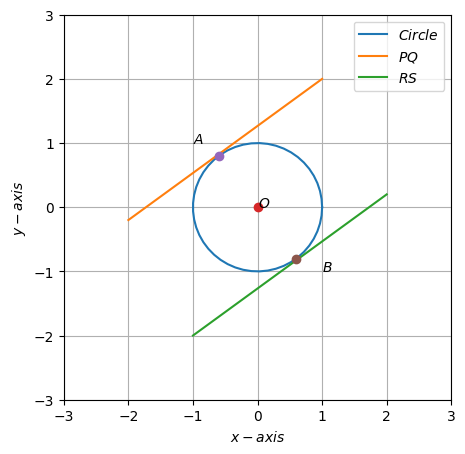
\includegraphics[width=\columnwidth]{fig/10.10.2.4.png}                       
	\caption{}               
	\label{10.10.2.4}
\end{figure}

\end{document}

